%\documentclass[11pt,addpoints,tikz]{exam}
\usepackage[utf8]{inputenc}
\usepackage[T1]{fontenc}
\usepackage{amsmath,amssymb,amsfonts,enumitem,graphicx,xcolor}
\usepackage{tikz}
\usetikzlibrary{arrows.meta,calc}
\usepackage{multicol}
\usepackage{draftwatermark}
\usepackage{eso-pic}

\newcommand\BackgroundPic{%
\put(0,0){%
\parbox[b][\paperheight]{\paperwidth}{%
\vfill
\centering

\includegraphics[width=\paperwidth,height=\paperheight,keepaspectratio]{Logo.png}%
\vfill}}}

% Uncomment the next line to produce the instructor key.
% \printanswers

\pagestyle{headandfoot}
\header{\textbf{Student Name:}}{\LARGE\textbf{Calculus I Exam}}{Limits, Derivatives, and Integrals}
\firstpageheader{\textbf{Student Name:}\\\textbf{Student Number:}\\\textbf{Period:}}{\LARGE\textbf{Calculus I Exam}}{%
  Limits, Derivatives, and Integrals\\\hspace*{1cm}Mr. Angerhofer\\
  \textbf{Date:\hspace*{15mm}}}
\headrule
\footrule
\footer{}{Page \thepage\ of \numpages}{}
\setlength{\columnsep}{1cm}
\renewcommand{\solutiontitle}{\noindent\textbf{Solution:}\enspace}

\begin{document}
\AddToShipoutPicture{\BackgroundPic}

\ifprintanswers
  \begin{center}
    \textcolor{red}{\Huge\textbf{SOLUTIONS GUIDE}}
  \end{center}
\else
  \begin{center}
    \fbox{\fbox{\parbox{5.8in}{\centering
      \begin{enumerate}[leftmargin=*,itemsep=2pt]
        \item Answer the questions in the spaces provided. If you run out of room, ask for scratch paper.
        \item Work must be shown for partial credit and is required when a question asks for an explanation.
        \item The exam has a no-calculator portion followed by acalculator portion.
        \item If you have a question, raise your hand and wait for the teacher.
      \end{enumerate}
    }}}
  \end{center}
\fi

\begin{center}
  \textbf{Total: 62 points \hspace{1cm} \hspace{1cm} \textbf{Time: 60 minutes}}
\end{center}

\begin{questions}

\section*{Part I: No Calculator }

\question[3] Use the table to evaluate the limit. Explain briefly how the table supports your answer.
\[
\begin{array}{c|ccccc}
x&1.9&1.99&2&2.01&2.1\\ \hline
f(x)&3.91&3.991&\text{undefined}&4.009&4.09
\end{array}
\qquad
\lim_{x\to 2}f(x)=\underline{\hspace{1.2in}}
\]

\question Use the graph of $f(x)$ below to answer the following questions.
\begin{center}
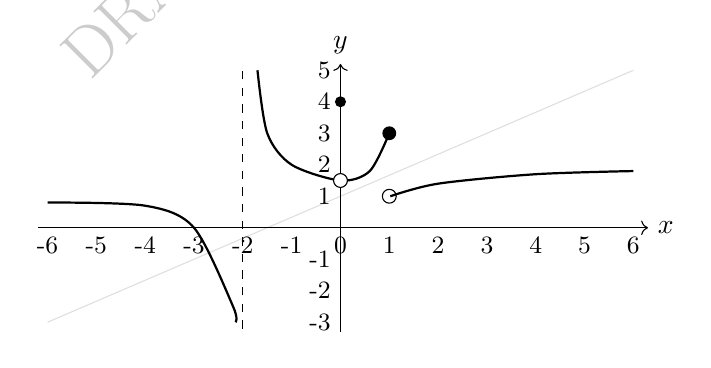
\begin{tikzpicture}[x=0.62cm,y=0.40cm]
  \draw[step=1,gray!25] (-6,-3)--(6,5);
  \draw[->] (-6.2,0)--(6.3,0) node[right] {$x$};
  \draw[->] (0,-3.3)--(0,5.2) node[above] {$y$};
  \draw[thick] plot[smooth] coordinates {(-6,0.8) (-4,0.7) (-3,0) (-2.2,-2.5) (-2.15,-3)};
  \draw[dashed] (-2,-3.2)--(-2,5);
  \draw[thick] plot[smooth] coordinates {(-1.7,5) (-1.5,3) (-1,2) (0,1.5) (0.6,1.8) (1,3)};
  \fill (0,4) circle (2pt);
  \draw[fill=white] (0,1.5) circle (2.5pt);
  \draw[fill=white] (1,1) circle (2.5pt);
  \fill (1,3) circle (2.5pt);
  \draw[thick] plot[smooth] coordinates {(1.02,1) (2,1.4) (4,1.7) (6,1.8)};
  \foreach \x in {-6,-5,-4,-3,-2,-1,0,1,2,3,4,5,6} \node[below] at (\x,0) {\small \x};
  \foreach \y in {-3,-2,-1,1,2,3,4,5} \node[left] at (0,\y) {\small \y};
\end{tikzpicture}
\end{center}
\begin{parts}
\part[1] $\displaystyle\lim_{x\to\infty}f(x) = $
\part[1] $\displaystyle\lim_{x\to-2^+}f(x) = $
\part[1] $\displaystyle\lim_{x\to-2^-}f(x) = $
\part[1] $\displaystyle\lim_{x\to-2}f(x) = $
\part[1] $\displaystyle\lim_{x\to0}f(x) = $
\part[1] $\displaystyle\lim_{x\to1^-}f(x) = $
\part[2] Is $f(x)$ continuous at $x=0$? Use the definition of continuity to explain why or why not.
\begin{solution}[1cm]
  False, we would have to jump from the hole to point $(0,4)$ which makes it not conitnuous.
\end{solution}
\end{parts}


\question Let

\[
\begin{cases}
f(x)= 
x^2-4, & x \leq 2,\\
3x-6, & x>2.
\end{cases}
\]
\begin{parts}
\part[3] Find \(\displaystyle\lim_{x\to2^-}f(x)\) and \(\displaystyle\lim_{x\to2^+}f(x)\).
\begin{solution}[2cm]
  \(\displaystyle\lim_{x\to2^-}f(x) = 0\) and \(\displaystyle\lim_{x\to2^+}f(x) = 0\)
\end{solution}
\part[2] Is \(f\) continuous at \(x=2\)? Use the definition of continuity to justify your answer.
\begin{solution}[2cm]
  Yes, because \(\displaystyle\lim_{x\to2^-}f(x) = \displaystyle\lim_{x\to2^+}f(x) = f(2) = 0\)
\end{solution}
\end{parts}

\question Suppose \(\displaystyle\lim_{x\to c}f(x)=5\) and
\(\displaystyle\lim_{x\to c}g(x)=-2\). Find each limit.
\begin{parts}
\part[1] \(\displaystyle\lim_{x\to c}[2f(x)-3g(x)]\)
\begin{solution}[1cm]
  \(\displaystyle\lim_{x\to c}[2f(x)-3g(x)] = 2(5) - 3(-2) = 10 + 6 = 16\)
\end{solution}
\part[1] \(\displaystyle\lim_{x\to c}\frac{g(x)}{f(x)}\)
\begin{solution}[1cm]
  \(\displaystyle\lim_{x\to c}\frac{g(x)}{f(x)} = \frac{-2}{5} = -\frac{2}{5}\)
\end{solution}
\part[1] \(\displaystyle\lim_{x\to c}[f(x)g(x)]\)
\begin{solution}[1cm]
  \(\displaystyle\lim_{x\to c}[f(x)g(x)] = (5)(-2) = -10\)
\end{solution}
\end{parts}

\question Find each limit algebraically, if it exists.
\begin{parts}
\part[2] \(\displaystyle\lim_{x\to4}\frac{x^2-16}{x-4}\)
\begin{solution}[3cm]
  \(\displaystyle\lim_{x\to4}\frac{x^2-16}{x-4} = \displaystyle\lim_{x\to4}\frac{(x-4)(x+4)}{x-4} = \displaystyle\lim_{x\to4}(x+4) = 8\)
\end{solution}
\part[2] \(\displaystyle\lim_{x\to\infty}\frac{6x^2-x+1}{2x^2+5}\)
\begin{solution}[2cm]
  \(\displaystyle\lim_{x\to\infty}\frac{6x^2-x+1}{2x^2+5} = \displaystyle\lim_{x\to\infty}\frac{6-\frac{1}{x}+\frac{1}{x^2}}{2+\frac{5}{x^2}} = \frac{6}{2} = 3\)
\end{solution}
\end{parts}

\question[3] Find the $x$-values, if any, at which $f(x)$ is not continuous. 

\[
f(x)=
\begin{cases}
x^2-2, & x\leq 1,\\[2pt]
\dfrac{x^2-4}{x-2}, & x>1.
\end{cases}
\]
\begin{solution}[2cm]
  $f(x)$ is not continuous at $x=2$ because the limit from the left does not equal the limit from the right.
\end{solution}


\question[2] Which of the following expressions equals $2$ for the graph shown below?
\begin{center}
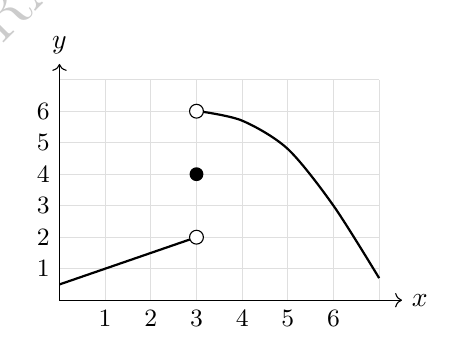
\begin{tikzpicture}[x=0.58cm,y=0.40cm]
  \draw[step=1,gray!25] (0,0) grid (7,7);
  \draw[->] (0,0)--(7.5,0) node[right] {$x$};
  \draw[->] (0,0)--(0,7.5) node[above] {$y$};
  \draw[thick] (0,0.5)--(3,2);
  \draw[thick] plot[smooth] coordinates {(3.05,6) (4,5.7) (5,4.8) (6,3) (7,0.7)};
  \draw[fill=white] (3,2) circle (2.5pt);
  \draw[fill=white] (3,6) circle (2.5pt);
  \fill (3,4) circle (2.5pt);
  \foreach \x in {1,2,3,4,5,6} \node[below] at (\x,0) {\small \x};
  \foreach \y in {1,2,3,4,5,6} \node[left] at (0,\y) {\small \y};
\end{tikzpicture}
\end{center}
\begin{multicols}{2}
\begin{enumerate}[label=(\Alph*)]
\item $f(3)$
\item $\displaystyle\lim_{x\to3^-}f(x)$
\item $\displaystyle\lim_{x\to3^+}f(x)$
\item $\displaystyle\lim_{x\to3}f(x)$
\end{enumerate}
\end{multicols}
\begin{solution}[1cm]
  The correct answer is (B) $\displaystyle\lim_{x\to3^-}f(x)$ because the limit from the left approaches $2$.
\end{solution}


\question[2] For $x<0$, the line $y=3$ is an asymptote of the graph of a function $f$. Which statement must be true?
\begin{multicols}{2}
\begin{enumerate}[label=(\Alph*)]
\item $f(x)\ne3$ for $x<0$
\item $\displaystyle\lim_{x\to-\infty}f(x)=3$
\item $\displaystyle\lim_{x\to\infty}f(x)=3$
\item $\displaystyle\lim_{x\to3}f(x)=\infty$
\end{enumerate}
\end{multicols}
\begin{solution}[1cm]
  The correct answer is (B) $\displaystyle\lim_{x\to-\infty}f(x)=3$ because an asymptote indicates that the function approaches that value as $x$ goes to negative infinity.
\end{solution}

\question[2] If $f$ is continuous on the closed interval $[2,5]$, $f(2)=-3$, and $f(5)=4$, which statement must be true?
\begin{multicols}{2}
\begin{enumerate}[label=(\Alph*)]
\item $f(c)=2$ for some $c\in(-3,4)$
\item $f(c)\ne1$ for every $c\in(2,5)$
\item $f(c)=0$ for some $c\in(-3,4)$
\item $f(c)=2$ for some $c\in(2,5)$
\end{enumerate}
\end{multicols}
\begin{solution}[1cm]
  The correct answer is (D) $f(c)=2$ for some $c\in(2,5)$ because by the Intermediate Value Theorem, since $f(2)=-3$ and $f(5)=4$, there must be some value $c$ in the interval $(2,5)$ where $f(c)=2$.
\end{solution}

\newpage
\section*{Part II: Calculator Allowed }

\question The velocity \(v(t)\), in feet per second, of a car is represented by the graph below.
\begin{center}
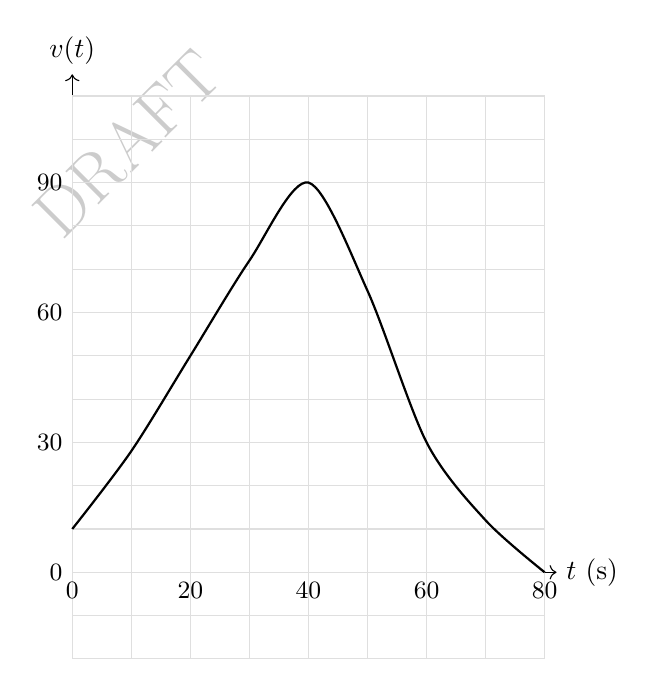
\begin{tikzpicture}[x=0.075cm,y=0.055cm]
  \draw[->] (0,0)--(82,0) node[right] {$t$ (s)};
  \draw[->] (0,-20)--(0,115) node[above] {$v(t)$};
  \draw[step=10,gray!25] (0,-20) grid (80,110);
  %\draw[thick] (0,10)--(20,50)--(40,90)--(60,30)--(80,0);
  \foreach \x in {0,20,40,60,80} \node[below] at (\x,0) {\small \x};
  \foreach \y in {0,30,60,90} \node[left] at (0,\y) {\small \y};
  \draw[thick] plot[smooth] coordinates {(0,10) (10,28) (20,50) (30,72) (40,90) (50,65) (60,30) (70,12) (80,0)};

\end{tikzpicture}
\end{center}
\begin{parts}
\part[2] Estimate the instantaneous rate of change of \(v\) at \(t=60\) by drawing a tangent line and using a difference quotient.
\begin{solution}[2cm]
  The instantaneous rate of change at \(t=60\) can be estimated by drawing a tangent line at that point and calculating the slope. For example, if the tangent line passes through points (60,30) and (70,12), the slope would be \(\frac{12-30}{70-60} = \frac{-18}{10} = -1.8\) ft/s².
\end{solution}
\part[1] What does the rate of change in part (a) represent in this context?
\begin{solution}[1cm]
  The rate of change represents the acceleration of the car at \(t=60\) seconds, indicating how quickly the velocity is changing at that moment.
\end{solution}
\part[2] Estimate the distance traveled from \(t=20\) to \(t=60\) by counting geometric areas.
\begin{solution}[2cm]
  The distance traveled can be estimated by calculating the area under the velocity curve from \(t=20\) to \(t=60\). This can be done by approximating the area using geometric shapes (triangles and rectangles) or using numerical integration methods.
\end{solution}
\part[3] Estimate the total distance traveled from \(t=0\) to \(t=80\) by using the Trapezoid Rule with four subintervals.
\begin{solution}[4cm]
  To estimate the total distance traveled from \(t=0\) to \(t=80\) using the Trapezoid Rule with four subintervals, divide the interval into four equal parts: [0,20], [20,40], [40,60], and [60,80]. Calculate the area of each trapezoid formed by the velocity values at the endpoints of each subinterval and sum them up to get the total distance.
\end{solution}
\end{parts}

\question[5] For \(s(t)=-t^2+12t+5\), find the average velocity on the interval
\([2,2.1]\). Then state the instantaneous velocity at \(t=2\) by taking the appropriate limit.
\begin{solution}[4cm]
  The average velocity on the interval \([2,2.1]\) is calculated as:
  \[
  \text{Average velocity} = \frac{s(2.1) - s(2)}{2.1 - 2} = \frac{(-2.1^2 + 12(2.1) + 5) - (-2^2 + 12(2) + 5)}{0.1}
  \]
  Calculate \(s(2)\) and \(s(2.1)\):
  \[
  s(2) = -4 + 24 + 5 = 25, \quad s(2.1) = -4.41 + 25.2 + 5 = 25.79
  \]
  Thus,
  \[
  \text{Average velocity} = \frac{25.79 - 25}{0.1} = \frac{0.79}{0.1} = 7.9 \text{ m/s}
  \]
  
  The instantaneous velocity at \(t=2\) is found by taking the derivative of \(s(t)\):
  \[
  v(t) = s'(t) = -2t + 12
  \]
  Evaluating at \(t=2\):
  \[
  v(2) = -4 + 12 = 8 \text{ m/s}
  \]
\end{solution}

\question A particle moves along a line with position
\[
s(t)=0.4t^3-3t^2+8t+2
\]
for \(0\leq t\leq 6\), where \(s\) is measured in meters and \(t\) in seconds.
\begin{parts}
\part[2] Find the particle's average velocity on \(2\leq t\leq5\).
\begin{solution}[4cm]
  The average velocity is given by:
  \[
  \text{Average velocity} = \frac{s(5) - s(2)}{5 - 2}
  \]
  Calculate \(s(2)\) and \(s(5)\):
  \[
  s(2) = 0.4(8) - 3(4) + 8(2) + 2 = 3.2 - 12 + 16 + 2 = 9.2
  \]
  \[
  s(5) = 0.4(125) - 3(25) + 8(5) + 2 = 50 - 75 + 40 + 2 = 17
  \]
  
  Thus,
  \[
  \text{Average velocity} = \frac{17 - 9.2}{3} = \frac{7.8}{3} = 2.6 \text{ m/s}
  \]
  \end{solution}
\part[2] Use the calculator to find the instantaneous velocity at \(t=3\), and interpret its sign.
\begin{solution}[4cm]
  The instantaneous velocity is given by the derivative of \(s(t)\):
  \[
  v(t) = s'(t) = 1.2t^2 - 6t + 8
  \]
  Evaluating at \(t=3\):
  \[
  v(3) = 1.2(9) - 6(3) + 8 = 10.8 - 18 + 8 = 0.8 \text{ m/s}
  \]
  
  The positive sign indicates that the particle is moving in the positive direction along the line at \(t=3\).
  \end{solution}
\end{parts}

\question The graph of \(f\) is modeled by
\[
f(x)=\frac{x^2-5x+6}{x-2}.
\]
\begin{parts}
\part[2] Use algebra to identify any discontinuity(s).
\begin{solution}[2cm]
  The function \(f(x)\) can be factored as:
  \[
  f(x) = \frac{(x-2)(x-3)}{x-2}
  \]
  For \(x \neq 2\), this simplifies to \(f(x) = x - 3\). However, at \(x=2\), the function is undefined, indicating a discontinuity at \(x=2\).
\end{solution}

\part[2] Use a graphing calculator to display the graph near the discontinuity and state the value of \(\displaystyle\lim_{x\to2}f(x)\).
\begin{solution}[2cm]
  Using a graphing calculator, we can see that as \(x\) approaches 2 from either side, the function values approach 1. Therefore,
  \[
  \lim_{x\to2}f(x) = 1.
  \]
\end{solution}
\part[1] Find the horizontal asymptote, if one exists.
\begin{solution}[1cm]
  As \(x\) approaches infinity, the function behaves like \(f(x) = x - 3\), which does not approach a finite value. Therefore, there is no horizontal asymptote.
\end{solution}
\end{parts}

\question[4] Find \(a\) and \(b\) so that the function is continuous for all real \(x\):
\[
f(x)=
\begin{cases}
2x+a, & x<-1,\\
ax+b, & -1\leq x\leq3,\\
4x-b, & x>3.
\end{cases}
\]
Show the two equations you use and solve the resulting system.
\begin{solution}[5cm]
  To ensure continuity at \(x=-1\):
  \[
  \lim_{x \to -1^-} f(x) = \lim_{x \to -1^+} f(x)
  \]
  \[
  2(-1) + a = a(-1) + b \implies -2 + a = -a + b \implies 2a - b = 2 \quad (1)
  \] 
  To ensure continuity at \(x=3\):
  \[
  \lim_{x \to 3^-} f(x) = \lim_{x \to 3^+} f(x)
  \]
  \[
  a(3) + b = 4(3) - b \implies 3a + b = 12 - b \implies 3a + 2b = 12 \quad (2)
  \]
  Solving the system of equations (1) and (2):
  \[
  \begin{cases}
  2a - b = 2 \\
  3a + 2b = 12
  \end{cases}
  \]
  From equation (1): \(b = 2a - 2\)
  Substituting into equation (2):
  \[
  3a + 2(2a - 2) = 12 \implies 3a + 4a - 4 = 12 \implies 7a = 16 \implies a = \frac{16}{7}
  \]
  Then, \(b = 2(\frac{16}{7}) - 2 = \frac{32}{7} - 2 = \frac{32 - 14}{7} = \frac{18}{7}\)
  Therefore, \(a = \frac{16}{7}\) and \(b = \frac{18}{7}\).
\end{solution}

\question[4] Verify that the Intermediate Value Theorem applies to
\(p(x)=x^3-4x+1\) on \([0,2]\). Use a calculator to locate one value of \(c\) in \((0,2)\) for which \(p(c)=0\), rounded to three decimal places.

%\question[4] The rate of change of water depth in a tank is modeled by
%\[
%r(t)=\frac{18}{t+2}+0.5t
%\]
%liters per minute for \(0\leq t\leq10\). Use a calculator and the Trapezoid Rule with five equal subintervals to estimate the total change in the amount of water during the first ten minutes. Is the estimate an overestimate or an underestimate? Explain using the shape of the graph.

\end{questions}
\end{document}
